\section{Resolución Problema 5}
La conversión de números binarios a decimales es un proceso fundamental en el campo de la informática y las matemáticas. Para obtener la conversión de binario a decimal, se empleó la siguiente fórmula inicialmente:
\begin{equation}
D = \sum_{i=0}^{n-1} (B[i] \cdot 2^i) 
\end{equation} 
En esta fórmula, cada dígito binario $B [i]$ se multiplica por la potencia correspondiente de la base binaria, que es 2. El exponente $i$ varía desde 0 hasta $n-1$, donde $n$ representa el número total de dígitos en la representación binaria. Al sumar estos productos, se obtiene el número decimal $D$, que es el resultado de la conversión. 
\subsection{\textbf{Descripción del problema:}}
\begin{enumerate}
\item Tomar el número binario de $n$ bits como entrada.
  \item Recorrer cada bit del número binario de izquierda a derecha.
  \item Para cada bit, multiplicar su valor (0 o 1) por la potencia de 2 correspondiente a su posición.
  \item Sumar todos los resultados de las multiplicaciones realizadas en el paso anterior.
  \item El resultado obtenido es el equivalente en decimal del número binario de entrada.
\end{enumerate}
\subsection{\textbf{Definición de solución:}}
La solución para convertir un número binario a decimal se basa en la siguiente fórmula:

\begin{equation}
D = \sum_{i=0}^{n-1} (B[i] \cdot 2^i)
\end{equation}

En esta fórmula, se multiplican los bits del número binario $B$ por las potencias correspondientes de 2, según su posición en la secuencia. Luego, se suman los productos obtenidos. El resultado de esta suma es el número decimal equivalente al número binario.
\subsection{\textbf{Diseño de la solución:}}
Seguidamente se muestra, un diagrama de flujo que fue de vital importancia para el desarrolo del programa en java:
\subsection{\textbf{Desarrollo de la solución:}}
En esta sección se comienza solicitando al usuario que ingrese un número binario válido, compuesto únicamente por los dígitos 0 y 1.

\begin{lstlisting}[style=javaStyle]
        Scanner sc = new Scanner(System.in);
// Se le pide al usuario que ingrese un número binario.
    System.out.println("Ingrese por favor el número binario (solo están permitidos 0 y 1): ");
    String binario = sc.nextLine();
  
\end{lstlisting}
Se llama a validarBin para verificar si el número binario ingresado es válido. Recorre cada dígito y verifica si es 0 o 1. Devuelve false si encuentra otro dígito, indicando que el número es inválido, y true si todos los dígitos son 0 o 1, continuando la ejecución.
\begin{lstlisting}[style=javaStyle] 
    
// Condición para que solo se puedan agregar los caracteres 0 y 1.
        if (!validarBin(binario)) 
            System.out.println("Error: El número binario ingresado contiene dígitos no válidos.");
            return;
     
\end{lstlisting}

Después de la validación, se llama a convertirBin para convertir el número binario a decimal. Esta función toma el número binario como entrada y devuelve su equivalente en decimal.
\begin{lstlisting}[style=javaStyle] 
    int decimal = convertirBin(binario);
    System.out.println("La conversión a número decimal es: " + decimal);
\end{lstlisting}
Se llama al método convertirBin() pasando el número binario como argumento. Este método realiza la conversión del número binario a decimal utilizando un bucle.
\begin{lstlisting} [style=javaStyle] 
    for (int i = 0; i < longitud; i++) {
        char digito = binario.charAt(i);
        int valor = Character.getNumericValue(digito);
        decimal += valor * Math.pow(2, exponente);
        exponente--;
    }

    return decimal;

\end{lstlisting}
Se define un método llamado validarBin que se utiliza para validar si un número binario solo contiene los caracteres '0' y '1'.  El método se utiliza para validar si un número binario es válido antes de realizar la conversión a decimal.
\begin{lstlisting} [style=javaStyle] 
}

// Metodo para validar si un número binario solo contiene los caracteres 0 y 1.
public static boolean validarBin(String binario) {
    for (int i = 0; i < binario.length(); i++) {
        char digito = binario.charAt(i);
        if (digito != '0' && digito != '1') {
            return false;
        }
    }
    return true;
  }
}
\end{lstlisting}

\subsection{\textbf{Depuración y pruebas:}}
\begin{figure}[h!]
    \centering
    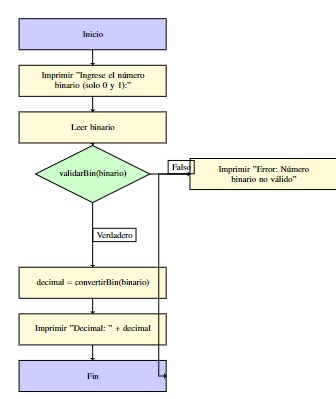
\includegraphics[width = 7.5 cm]{LaTeX/latex-imagenes/fig.1.jpeg}
    \caption{Depuración del código en java del programa binario a decimal.}
    \label{fig:DepuraciónCodigo}
\end{figure}

\begin{figure}[h!]
    \centering
    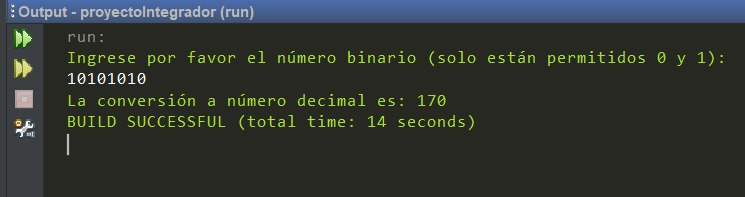
\includegraphics[width = 7.5 cm]{LaTeX/latex-imagenes/fig.2.jpeg}
    \caption{Tabla de conversión de numero binaria a decimlal.}
    \label{fig:DepuraciónCodigo}
\end{figure}